\section{Results}
\label{sec:results}

All numbers in this section come from the evaluation on the MIT-BIH test set (DS2) fixed in the analysis plan (1,195 windows, 22 patients) unless stated otherwise, and the tables and figures are generated from the result files by the scripts in the supplementary release. Adapter values are means of three training seeds. Intervals are 95\% patient-cluster bootstrap limits.

The subsections answer the three research questions in turn: what the latent lever costs relative to the others (RQ1), what it gives up or gains in the decision (RQ2), and what can still be read back from the message (RQ3). Each comparison is against the strongest text arm available for the question: calibrated compact text for accuracy against listing every event, and filtered text for any claim that the latent channel is worth building. Section~\ref{sec:discussion} combines the three answers into a selection rule.

\subsection{RQ1: Cost of the Interface}
At a single event the adapter has nothing to save. Its four tokens replace about 57 tokens of compact text, but the fixed scaffold dominates the prompt (end-to-end lengths of 486 and 458 tokens for the two arms in the single-event study), and time to first token is unchanged. The advantage appears only when a prompt carries many events (Table~\ref{tab:cost}). Text grows by about 60 tokens per event whereas the adapter adds four, so the adapter's prompt-processing time stays near 183~ms from 1 to 50 events while the time of compact text rises to 845~ms. Time to the tier token falls less because the decision includes generating the first answer tokens, which costs the same in both arms.

\begin{table}[t]
\caption{Cost of the adapter relative to compact text (batch one, median over 21 windows per $N$).}
\label{tab:cost}
\centering
\small
\adjustbox{max width=\linewidth}{\begin{tabular}{rrrrrr}
\toprule
$N$ & Tokens (text / adapter) & TTFT ms (text / adapter) & TTFT & Decision & Context MB \\
\midrule
1 & 576 / 516 & 181 / 184 & 0\% & $+1\%$ & --- \\
5 & 811 / 532 & 197 / 182 & $-8\%$ & $-1\%$ & $-$36 \\
10 & 1105 / 553 & 241 / 183 & $-24\%$ & $-4\%$ & $-$79 \\
20 & 1694 / 593 & 360 / 181 & $-50\%$ & $-14\%$ & $-$177 \\
50 & 3457 / 713 & 845 / 183 & $-78\%$ & $-36\%$ & $-$460 \\
\bottomrule
\end{tabular}
}
\end{table}

\begin{figure}[t]
\centering
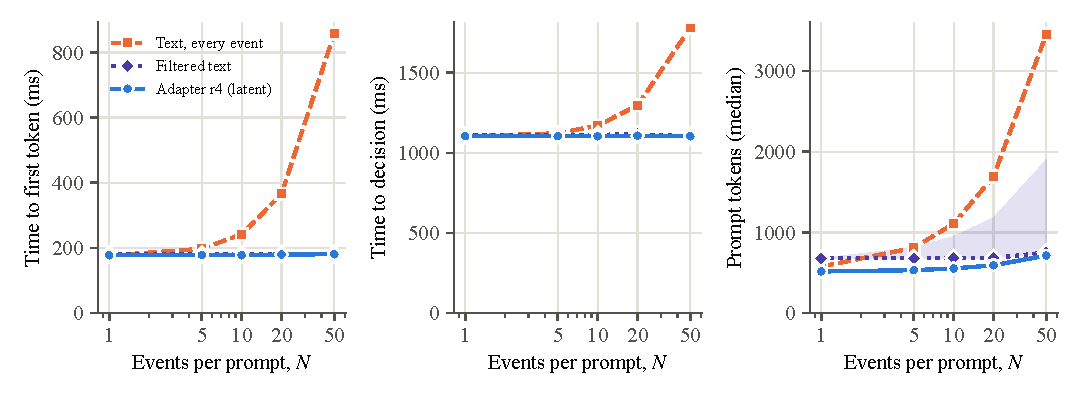
\includegraphics[width=\linewidth]{figures/fig_cost.pdf}
\caption{Cost of the three interfaces against the number of events per prompt (batch one, median of 21 windows per $N$). The shaded band in the right panel is the 90th percentile of the filtered prompt: its length depends on content, whereas the adapter's depends only on $N$. Time to decision is almost identical for filtered text and the adapter.}
\label{fig:cost}
\end{figure}

\textbf{Serving.} Single-request timing flatters neither arm because nothing is reused. Under batching, text that lists every event could not be served at a batch of eight at any $N \ge 10$, nor at a batch of four at 50 events, on the 12~GB card, whereas the adapter fitted every configuration with a peak of about 10~GB. Against A-filtered, the adapter was within about 5\% in time and throughput for single requests, with 3 to 12\% less energy per decision and overlapping interquartile ranges. Once requests were batched, its median throughput was 10 to 30\% higher and its median energy per decision 12 to 28\% lower (Table~\ref{tab:serving}), but at a batch of four the interquartile ranges of the two arms overlap for throughput at 10 and 50 events and for energy at 50 events, because the cost of filtered text varies with content. Filtered text fitted only some batches: 3 of 6 at a batch of eight for every $N$, and 12 of 15 at a batch of four for 50 events. Its figures for those cells describe only the batches that fit, which are its shortest prompts, so they favour filtered text and are not a measurement of filtered text at that batch size. These serving results come from one GPU, one serving framework and one adapter, and we read them as a promising result for this setup rather than a general advantage. Prefix caching shortened every arm's prefill and did not change the ranking.

\begin{table}[t]
\caption{Decisions per second and GPU board energy per decision when requests are batched: median (interquartile range) over all measurements of the cell (final adapter, first training seed). ``Does not fit'': the batch exceeds the 12~GB memory cap. $^\ast$Only the stated number of batches fitted; the values describe that subset (the shortest prompts) and not the arm at that batch size.}
\label{tab:serving}
\centering
\small
\adjustbox{max width=\linewidth}{\begin{tabular}{rrccc}
\toprule
$N$ & Batch & Adapter & Text, all events & Filtered text \\
\midrule
10 & 1 & 0.98 (0.94--1.02)/s; 83 (77--87) J & 0.92 (0.82--0.97)/s; 111 (103--120) J & 0.97 (0.83--1.02)/s; 95 (86--105) J \\
10 & 4 & 3.19 (2.87--3.32)/s; 38 (38--42) J & 2.23 (2.19--2.36)/s; 65 (64--67) J & 2.80 (2.11--2.94)/s; 49 (45--70) J \\
10 & 8 & 4.72 (4.50--4.86)/s; 33 (31--33) J & does not fit & 3.63 (3.48--3.77)/s; 43 (42--44) J$^\ast$ 3/6 \\
20 & 1 & 0.98 (0.91--1.05)/s; 81 (77--88) J & 0.85 (0.78--0.88)/s; 134 (129--143) J & 0.97 (0.85--1.01)/s; 92 (83--108) J \\
20 & 4 & 3.17 (3.10--3.30)/s; 39 (38--40) J & 1.70 (1.69--1.74)/s; 92 (90--92) J & 2.49 (1.87--2.72)/s; 54 (47--77) J \\
20 & 8 & 4.55 (4.13--4.75)/s; 33 (32--36) J & does not fit & 4.00 (3.95--4.11)/s; 38 (38--39) J$^\ast$ 3/6 \\
50 & 1 & 1.00 (0.87--1.06)/s; 89 (83--96) J & 0.60 (0.56--0.61)/s; 232 (227--244) J & 0.96 (0.83--1.00)/s; 92 (85--110) J \\
50 & 4 & 2.79 (2.49--2.92)/s; 48 (46--52) J & does not fit & 2.25 (1.78--2.89)/s; 63 (47--83) J$^\ast$ 12/15 \\
50 & 8 & 4.11 (3.97--4.27)/s; 38 (37--39) J & does not fit & 3.72 (3.66--3.79)/s; 43 (42--43) J$^\ast$ 3/6 \\
\bottomrule
\end{tabular}
}
\end{table}

\begin{figure}[t]
\centering
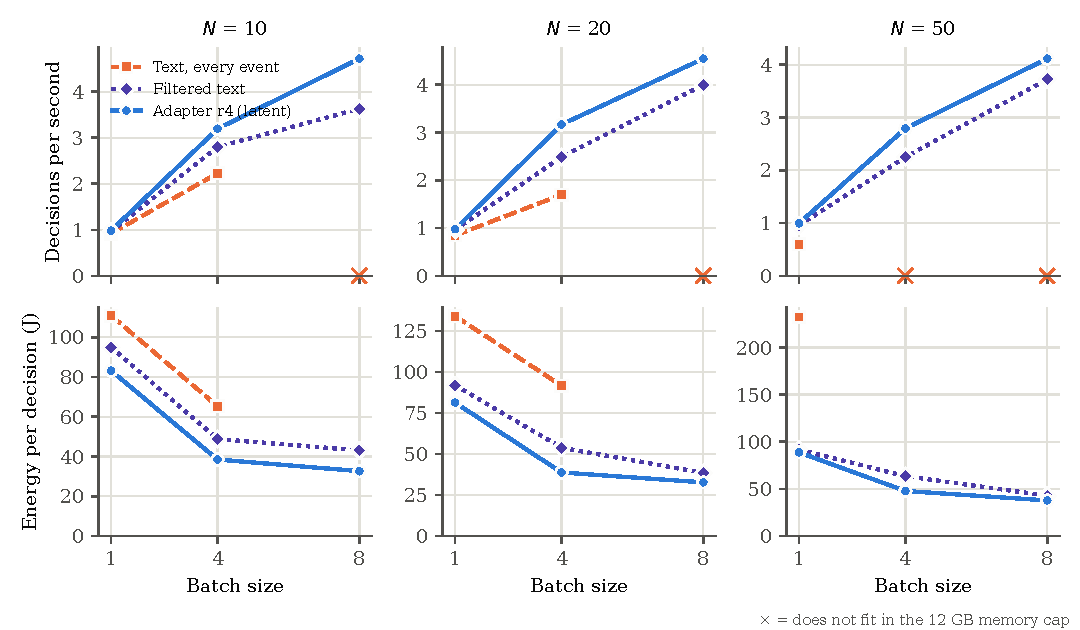
\includegraphics[width=\linewidth]{figures/fig_serving.pdf}
\caption{Throughput (top) and GPU energy per decision (bottom) when requests are batched, for 10, 20 and 50 events per prompt (final adapter, first training seed; medians). A cross marks a configuration that did not fit in the memory cap of the 12~GB card. Filtered text at batch eight is plotted from the batches that fit, which are its shortest prompts.}
\label{fig:serving}
\end{figure}

\subsection{RQ2: Accuracy}
\textbf{Against text that lists every event.} Default compact text falls from 0.97 balanced accuracy at one event to 0.48 to 0.56 at 10 to 50 events. Calibration recovers part of this (0.73 to 0.76) and is the fair comparison. The final adapter holds 0.81 to 0.84 at 5 to 50 events (Table~\ref{tab:accuracy}). Against calibrated text, the adapter was superior at 10 and 20 events (both $+0.10$, intervals excluding zero) and non-inferior at 5 and 50 events. At a single event, text was better (0.97 against 0.80), as expected from the cost analysis.

\begin{table}[t]
\caption{Balanced accuracy on class-balanced DS2 windows, and adapter minus calibrated text with 95\% patient-cluster intervals. Rule: the reference rule applied directly to the sender's outputs, 1 by construction and computed in microseconds; it is the ceiling of every channel and shows that the task itself does not need a language model (Section~\ref{sec:intro}). The adapter is superior at $N=10$ and 20 (interval above zero) and non-inferior at $N=5$ and 50 (lower limit above the margin of $-0.05$).}
\label{tab:accuracy}
\centering
\small
\begin{tabular}{rrrrrl}
\toprule
$N$ & Rule & Text & Text cal. & Adapter & Adapter $-$ cal. text [95\% CI] \\
\midrule
1 & 1.00 & 0.97 & 0.97 & 0.80 & --- \\
5 & 1.00 & 0.73 & 0.79 & 0.81 & $+0.03$ [$-0.04$, $+0.10$] \\
10 & 1.00 & 0.56 & 0.73 & 0.83 & $+0.10$ [$+0.03$, $+0.17$] \\
20 & 1.00 & 0.48 & 0.73 & 0.83 & $+0.10$ [$+0.01$, $+0.18$] \\
50 & 1.00 & 0.54 & 0.76 & 0.84 & $+0.08$ [$-0.02$, $+0.17$] \\
\bottomrule
\end{tabular}

\end{table}

\begin{figure}[t]
\centering
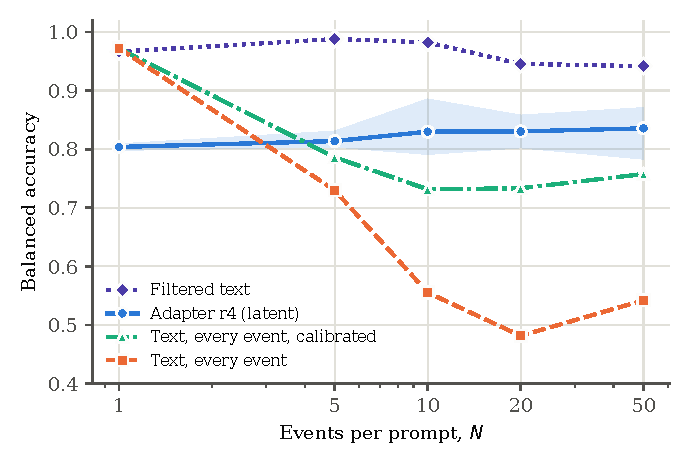
\includegraphics[width=0.85\linewidth]{figures/fig_accuracy.pdf}
\caption{Balanced accuracy against the number of events per prompt on the class-balanced test windows. The shaded band is the range of the three adapter seeds. Filtered text is the most accurate arm; text with every event listed degrades as events are added and calibration recovers only part of the loss.}
\label{fig:accuracy}
\end{figure}

\textbf{Why text with every event fails.} Two mechanisms account for most of the loss (Figure~\ref{fig:mechanisms}). Text misses urgent windows caused by a single high-confidence ventricular or fusion beat (a numeric threshold of 0.85 buried in a long list) far more often than windows caused by a run of abnormal beats. This is the clearest effect: text recalls 0.17 of such windows against 0.82 for the adapter. The position of the deciding beat points the way reported for long contexts \cite{liu2024lost,hsieh2024found}: text accuracy is lowest when that beat is in the middle third of the window (0.19, against 0.30 in the first and 0.38 in the last third). The evidence is weak. The middle group has 73 windows and its interval overlaps those of the other thirds (right panel of Figure~\ref{fig:mechanisms}), and the adapter shows a similar small dip (0.74 to 0.78 across positions). We report a position effect as suggested for text, not established, and not distinguishable from the adapter's.

\begin{figure}[t]
\centering
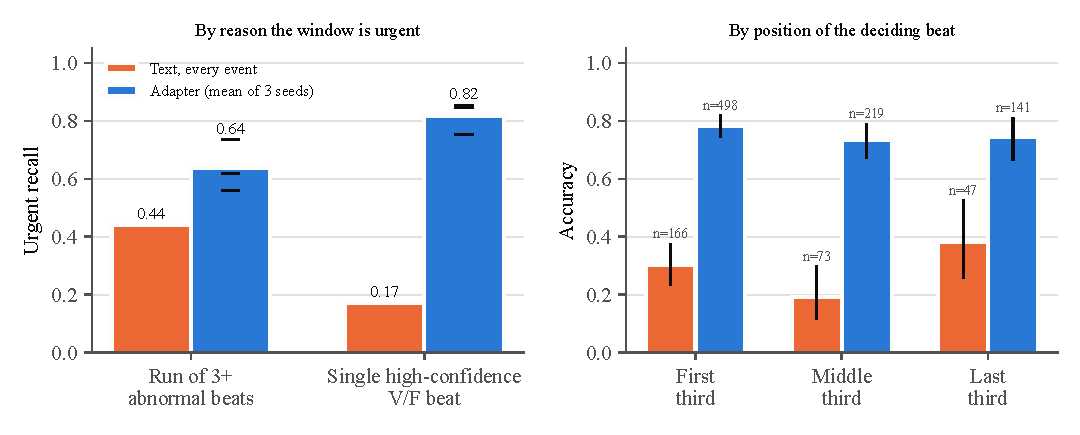
\includegraphics[width=0.65\linewidth]{figures/fig_mechanisms.pdf}
\caption{Urgent recall by the reason a window is urgent. Text with every event listed misses windows made urgent by a single high-confidence ventricular or fusion beat far more often than windows made urgent by a run; the adapter does not show this gap. Bars for the adapter are the mean of three seeds, with each seed's value marked. Right: accuracy on non-routine windows with $N \ge 10$ by the position of the window's most urgent beat; whiskers are 95\% Wilson intervals, and the adapter counts are windows times three seeds. This panel is exploratory (not in the analysis plan) and is computed by \texttt{scripts/position\_effect.py}.}
\label{fig:mechanisms}
\end{figure}

\textbf{False alarms.} The earlier adapter escalated about 11\% of routine windows, concentrated on windows with a normal beat of low classification confidence. The final adapter reduced the rate at every seed, by 44 to 80\% (about two thirds on average), to 3.6\% overall (0\% to 3.8\% at 50 events). Text raised none, because its error is the opposite one: it under-escalates urgent windows to priority. The adapter never called an urgent window routine in the 50-event confusion matrix.

\textbf{What the final adapter's gain comes from.} The final adapter differs from the earlier one in two ways: hard-negative routine windows in training, and three side inputs per event (heart rate, interval and run length). We retrained it without the side inputs, with three seeds and everything else identical (Table~\ref{tab:ablation}). The side inputs account for most of the improvement. Accuracy rose at every $N$ (by 0.03 to 0.05, with the interval excluding zero at 50 events) and false alarms fell from 8.6\% to 3.6\% in every seed. Hard negatives alone moved accuracy by about 0.01 and false alarms from 10.6\% to 8.6\%. The false-alarm reduction therefore comes mainly from giving the receiver the context to tell a low-confidence normal beat from a real event, not from the extra training examples.

\begin{table}[t]
\caption{Ablation of the final adapter (three seeds each): balanced accuracy, false alarms (FA) on routine windows, and the two contrasts with patient-cluster 95\% intervals. Hard negatives: hard-negative routine windows in training; side inputs: heart rate, interval and run length. The side-input contrast is clean (same windows and schedule); the hard-negative contrast is approximate, because the earlier adapter also used fewer training windows and a proportionally shorter schedule.}
\label{tab:ablation}
\centering
\footnotesize
\adjustbox{max width=\linewidth}{\begin{tabular}{lccccr}
\toprule
Recipe & $N$=5 & $N$=10 & $N$=20 & $N$=50 & FA \\
\midrule
r3 (neither) & 0.794 & 0.772 & 0.795 & 0.770 & 10.6\% \\
HN only & 0.788 & 0.786 & 0.802 & 0.781 & 8.6\% \\
r4 (HN + SI) & 0.814 & 0.830 & 0.830 & 0.836 & 3.6\% \\
SI: r4 $-$ HN only & $+0.03$ [$-0.02$, $+0.06$] & $+0.04$ [$-0.01$, $+0.11$] & $+0.03$ [$-0.01$, $+0.07$] & $+0.05$ [$+0.01$, $+0.11$] &  \\
HN: HN only $-$ r3 & $-0.01$ [$-0.04$, $+0.03$] & $+0.01$ [$-0.02$, $+0.05$] & $+0.01$ [$-0.04$, $+0.05$] & $+0.01$ [$-0.03$, $+0.05$] &  \\
\bottomrule
\end{tabular}
}
\end{table}

\textbf{Against text that lists only abnormal events.} A-filtered was more accurate than the adapter at every $N$ (Table~\ref{tab:filtered}), raised no false alarms, and for a single request matched it in time to first token and to decision within 1.5\%. Its cost depends on content: each listed abnormal beat adds about 68 tokens, so at 50 events its prompt is longer than the adapter's in half of the windows. The decision rule fixed in the analysis plan anticipated a filtered prompt that was cheaper but less accurate; applied literally it returned ``advantage holds'' because the filtered prompt turned out to be longer. We do not read it that way. Against filtered text, on this task, the latent interface has no accuracy advantage and no latency advantage for a single request.

\begin{table}[t]
\caption{Adapter against filtered text (default decoding) with patient-cluster intervals, and median prompt tokens (adapter / filtered).}
\label{tab:filtered}
\centering
\small
\begin{tabular}{rrrrr}
\toprule
$N$ & Adapter r4 & Filtered & Difference [95\% CI] & Tokens \\
\midrule
1 & 0.804 & 0.966 & --- & 516 / 679 \\
5 & 0.814 & 0.988 & $-0.17$ [$-0.22$, $-0.13$] & 532 / 679 \\
10 & 0.830 & 0.982 & $-0.15$ [$-0.19$, $-0.11$] & 553 / 682 \\
20 & 0.830 & 0.945 & $-0.12$ [$-0.16$, $-0.07$] & 593 / 683 \\
50 & 0.836 & 0.942 & $-0.11$ [$-0.17$, $-0.05$] & 713 / 750 \\
\bottomrule
\end{tabular}

\end{table}

\textbf{Against the annotations.} Scored against the database annotations instead of the sender's own rule, with a window counted as abnormal if any of its beats is annotated as not normal, the reference rule has sensitivity of 0.94 to 0.96 and specificity of only 0.46 to 0.64 across window sizes. The clinical ceiling is therefore set by perception and not by the interface: the final adapter tracked the reference (sensitivity 0.90 to 0.96 at 5 to 50 events), while default compact text missed more abnormal windows (0.77 to 0.79 at 10 to 50 events).

\textbf{Second sender.} The replication with a convolutional sender (validation accuracy 0.955 against a gate of 0.85) reproduced the pattern (Table~\ref{tab:second}). Text with every event listed fell as events were added while the adapter stayed at 0.77 to 0.82; the adapter was superior to calibrated text at 10 events and non-inferior at 20 and 50, but not at 5; false alarms were 1.3 to 2.1\%. A-filtered was again the most accurate arm except at 50 events, where it fell to 0.80 and the difference was inconclusive ($-0.01$ [$-0.09$, $+0.08$]). An exploratory look at those windows (40 per sender, so indicative only) suggests that this sender's urgent windows carry sparser, more borderline evidence, often one urgent beat among about 13 listed abnormal beats with a deciding confidence just above 0.85. Filtered text depends on how the sender's evidence is distributed, whereas the adapter did not change much.

\begin{table}[t]
\caption{Second sender (ResNet1D-RR): balanced accuracy on its own DS2 windows and adapter minus calibrated text (non-inferiority margin $-0.05$).}
\label{tab:second}
\centering
\footnotesize
\begin{tabular}{rrrrl}
\toprule
$N$ & Adapter & Text cal. & Filtered & Adapter $-$ cal. text [95\% CI] \\
\midrule
5 & 0.770 & 0.787 & 0.959 & $-0.02$ [$-0.11$, $+0.08$] \\
10 & 0.823 & 0.732 & 0.929 & $+0.09$ [$+0.02$, $+0.16$] \\
20 & 0.780 & 0.733 & 0.907 & $+0.05$ [$-0.03$, $+0.13$] \\
50 & 0.794 & 0.733 & 0.808 & $+0.06$ [$-0.02$, $+0.14$] \\
\bottomrule
\end{tabular}

\end{table}

\textbf{External confirmatory test.} The frozen system was evaluated once on a second database; the result is reported in Section~\ref{sec:incart}.

\subsection{RQ3: What Can Be Recovered}
\textbf{Single events.} Decoders trained on the training records and applied to the test records recovered the predicted beat label (accuracy 99.5\%) and tier (95\%; balanced accuracy 0.88) from the virtual tokens of the single-event adapters as well as from the 32-dimensional input, so the adapter loses nothing the vector holds.

\textbf{Every position.} For slots 0, 9, 19 and 49 of a 50-event window, label, tier and urgency decoded at the level of the input vector. Decoders are slot-specific: a decoder trained on slot 0 applied at slot 49 fell to 0.64 to 0.91, so an auditor needs a position-aware decoder.

\textbf{What the vector never carried.} The 32-dimensional context vector does not contain heart rate, interval or run length ($R^2$ about 0.3), so the earlier adapter could not carry them either. With the side inputs of the final adapter they are recoverable from the tokens (Table~\ref{tab:recover}). The decoder specified in advance was a small multilayer perceptron, and with it heart rate ($R^2$ 0.59 to 0.78) and interval (0.65 to 0.77) fall well short of the input (0.98 and 0.95), while the presence of a run of three abnormal beats is recovered at 0.93 to 0.98 balanced accuracy (0.53 to 0.61 for the earlier adapter, near chance). A linear decoder, fitted in the same analysis, recovers much more of the numeric fields from the same tokens (heart rate 0.95 to 0.97, interval 0.92 to 0.96). The multilayer decoder therefore understates what the tokens hold, and the information is held in a nearly linear form. We report both: the figure from the decoder specified in advance is the conservative one, and the linear figures are the better estimate of what an auditor could recover. On the second sender, heart rate and interval are recovered from every token slot at $R^2$ 0.89 to 0.94 with the decoder specified in advance. Signal quality is not carried by either sender.

\begin{table}[t]
\caption{Recoverability of each event's fields from its virtual tokens (final adapter, main sender), decoders trained on the training records and applied to the test records. Token columns give the range over slots 0 and 49 and three seeds. The multilayer perceptron was the decoder specified in advance; the linear decoder is reported for comparison.}
\label{tab:recover}
\centering
\footnotesize
\adjustbox{max width=\linewidth}{\begin{tabular}{lrrrr}
\toprule
Field & Input, MLP & Tokens, MLP & Input, linear & Tokens, linear \\
\midrule
Beat label (bal. acc.) & 0.99 & 0.95--0.98 & 0.99 & 0.99--1.00 \\
Tier (bal. acc.) & 0.95 & 0.92--0.95 & 0.91 & 0.90--0.94 \\
Urgency flag (bal. acc.) & 0.98 & 0.97--0.98 & 0.94 & 0.94--0.95 \\
Heart rate ($R^2$) & 0.98 & 0.59--0.78 & 1.00 & 0.95--0.97 \\
RR interval ($R^2$) & 0.95 & 0.65--0.77 & 0.98 & 0.92--0.96 \\
Run $\geq 3$ (bal. acc.) & 0.98 & 0.93--0.98 & 0.95 & 1.00--1.00 \\
\bottomrule
\end{tabular}
}
\end{table}

\textbf{Carried and used.} The ablation shows both directions. Without the side inputs, heart rate, interval and run length are not recoverable from the tokens at all ($R^2$ at most 0.09; run $\geq 3$ at 0.52 to 0.59, near chance); with them they are, and the receiver uses them, since they account for most of the accuracy gain and the false-alarm reduction (Table~\ref{tab:ablation}). Use is partial, however: urgent recall on windows made urgent by a run of three or more abnormal beats rose only from 0.61 to 0.64 when run length entered the tokens, against 0.44 for text.

\textbf{Pre-generation check.} For the single-event adapters, scores computed from the context vector alone flag inputs before generation: a tier decoder predicts the adapter's wrong answers (AUROC 0.89 to 0.97), and a Mahalanobis distance flags noise and powerline interference (0.99). This gives an inspection that does not need to read the tokens.

\textbf{Compression.} We retrained the adapter with one, two and eight virtual tokens per event in place of four (Table~\ref{tab:sweep}, Figure~\ref{fig:sweep}). A first sweep with one seed per setting suggested that a single token might suffice, so one and two tokens were repeated with three seeds each, under a rule fixed before training: a setting is free of accuracy cost only if it is non-inferior to four tokens (margin $-0.05$) at every $N$. Neither passed. With one token, one run in three failed to learn the task (0.49 to 0.55 at 5 to 50 events) while the other two matched four tokens, so the three-seed mean was 0.09 to 0.11 lower. With two tokens accuracy was within about 0.01 of four tokens at 5 to 20 events and 0.04 lower at 50, non-inferior only at 20 events, and false alarms were higher in every run (8.6\% on average against 3.6\%). Eight tokens, a single run, was no better than four. Each event's label, heart rate and run status remained recoverable from a single token, including from the one-token run that failed the task (label 0.96 to 0.99, heart-rate $R^2$ about 0.9 with the decoder specified in advance). Compression below four tokens per event therefore preserved what the tokens carry but made the receiver's use of it unreliable, and four tokens was the smallest setting at which every run was reliable. The saving would be modest in any case, because the scaffold dominates: at 50 events, 563 tokens at one token per event against 713 at four.

\begin{table}[t]
\caption{Virtual tokens per event: three seeds for $k$ = 1, 2 and 4 (means), one run for $k$ = 8. Tokens: prompt length at 50 events. $k-4$: difference from $k$ = 4 at the least favourable $N$ (50 in both cases), with its patient-cluster 95\% interval; NI: number of $N$ (of 5, 10, 20, 50) at which $k$ is non-inferior (margin $-0.05$). FA: false alarms on routine windows (seed ranges in the text). Label and HR $R^2$: recoverability from slot 0 with the decoder specified in advance (multilayer perceptron); the negative $R^2$ at $k$ = 8 is likely a decoder limit (32 principal components of a 20,480-dimensional slot).}
\label{tab:sweep}
\centering
\footnotesize
\adjustbox{max width=\linewidth}{\begin{tabular}{rrclcrrr}
\toprule
$k$ & Tokens & Bal. acc., $N$ = 5/10/20/50 & $k-4$ [95\% CI] & NI & FA & Label & HR $R^2$ \\
\midrule
1 & 563 & 0.70 / 0.72 / 0.75 / 0.73 & $-0.11$ [$-0.16$, $-0.06$] & 0/4 & 6.3\% & 0.97 & $0.87$ \\
2 & 613 & 0.80 / 0.82 / 0.83 / 0.80 & $-0.04$ [$-0.13$, $+0.03$] & 1/4 & 8.6\% & 0.95 & $0.81$ \\
4 & 713 & 0.81 / 0.83 / 0.83 / 0.84 & ref. & -- & 3.6\% & 0.96 & $0.71$ \\
8 & 913 & 0.77 / 0.80 / 0.78 / 0.80 & 1 run & -- & 6.1\% & 0.95 & $-0.62$ \\
\bottomrule
\end{tabular}
}
\end{table}

\begin{figure}[t]
\centering
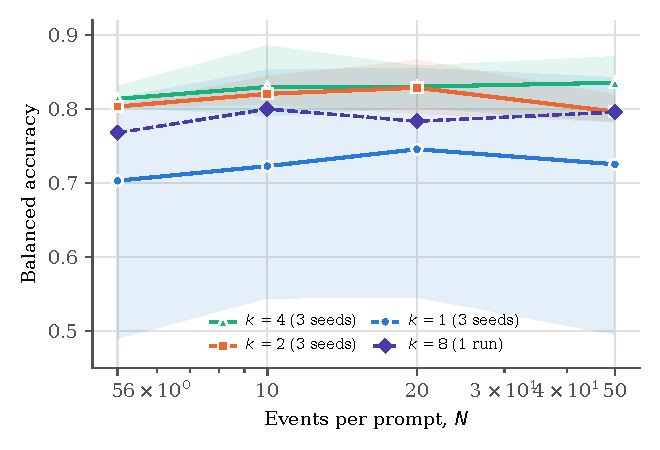
\includegraphics[width=0.7\linewidth]{figures/fig_sweep.pdf}
\caption{Balanced accuracy against the number of events for $k$ = 1, 2 and 4 virtual tokens per event (lines: mean of three seeds; bands: seed range) and $k$ = 8 (one run). The wide band at $k$ = 1 is one failed run.}
\label{fig:sweep}
\end{figure}

\subsection{External Confirmatory Test on INCART}
\label{sec:incart}
The DS2 test set informed several design iterations, so its results cannot confirm the final system. The confirmatory test is therefore a single run of the frozen system on a database that played no part in any decision. The St Petersburg INCART database has 75 half-hour recordings from 32 patients; after conversion to the same beat format (lead II, resampled from 257 to 360~Hz) it yields 175,777 accepted beats: 153,594 normal, 20,006 ventricular, 1,958 supraventricular and 219 fusion beats. A further 91 beats whose window fell outside the recording and 51 with an unmapped annotation symbol were excluded. The test set has 1,240 windows with every stratified cell filled (Table~\ref{tab:incartwindows}), and its hash was committed before any model output existed.

\begin{table}[t]
\caption{INCART test windows by number of events per prompt $N$ and reference tier. All stratified cells reached their quota.}
\label{tab:incartwindows}
\centering
\footnotesize
\adjustbox{max width=\linewidth}{\begin{tabular}{rrrrrrr}
\toprule
$N$ & Routine & Priority & Urgent & Stratified & Natural prevalence & Total \\
\midrule
1 & 60 & 60 & 60 & 180 & --- & 180 \\
5 & 60 & 60 & 60 & 180 & 100 & 280 \\
10 & 60 & 60 & 60 & 180 & 100 & 280 \\
20 & 60 & 60 & 60 & 180 & 100 & 280 \\
50 & 40 & 40 & 40 & 120 & 100 & 220 \\
All &  &  &  & 840 & 400 & 1240 \\
\bottomrule
\end{tabular}
}
\end{table}

The system under test was fixed in a manifest of file hashes before the run: the three final adapters (not retrained), the perception agent, the prompt and decoding code, and the calibration biases chosen on the DS1 validation windows and not re-tuned. Text arms were generated by stopping at the tier token, as decided after that choice was shown on DS2 to change no tier. The four hypotheses were tested in a fixed sequence at $\alpha = 0.05$, stopping at the first failure, with patient-cluster bootstrap intervals (20,000 resamples): \textbf{H1}, the adapter (three-seed mean) is non-inferior to calibrated compact text at $N$ = 10, 20 and 50 (margin $-0.05$, all three required); \textbf{H2}, it is superior at $N$ = 10 and 20; \textbf{H3}, it is non-inferior to calibrated filtered text at $N$ = 10, 20 and 50; \textbf{H4}, its median time to first token is lower than that of compact text at $N$ = 10, 20 and 50. Hypotheses after the first failure are reported descriptively as not tested in sequence.

\begin{table}[t]
\caption{Hypotheses on INCART, fixed in advance. Estimates are adapter minus calibrated text (H1, H2), adapter minus calibrated filtered text (H3), or the median relative difference in time to first token (H4), with 95\% intervals. H4 was not tested in sequence because H3 failed. $^\dagger$The time-to-first-token value at 50 events is the technical re-measurement under the memory cap (see text); the original value ($-0.97$) was distorted by memory paging.}
\label{tab:incarthyp}
\centering
\footnotesize
\adjustbox{max width=\linewidth}{\begin{tabular}{llrrll}
\toprule
Hypothesis & $N$ & Estimate & 95\% CI & Result & Status \\
\midrule
H1: non-inferior to calibrated text & 10 & $+0.08$ & [$+0.03$, $+0.15$] & pass & confirmed \\
 & 20 & $+0.09$ & [$+0.04$, $+0.15$] & pass &  \\
 & 50 & $+0.05$ & [$-0.04$, $+0.13$] & pass &  \\
H2: superior to calibrated text & 10 & $+0.08$ & [$+0.03$, $+0.15$] & pass & confirmed \\
 & 20 & $+0.09$ & [$+0.04$, $+0.15$] & pass &  \\
H3: non-inferior to calibrated filtered text & 10 & $-0.11$ & [$-0.17$, $-0.05$] & fail & not confirmed \\
 & 20 & $-0.11$ & [$-0.16$, $-0.06$] & fail &  \\
 & 50 & $-0.07$ & [$-0.15$, $-0.00$] & fail &  \\
H4: faster first token than text & 10 & $-0.27$ & [$-0.28$, $-0.26$] & pass & not tested in sequence \\
 & 20 & $-0.51$ & [$-0.52$, $-0.49$] & pass &  \\
 & 50$^\dagger$ & $-0.77$ & [$-0.78$, $-0.77$] & pass &  \\
\bottomrule
\end{tabular}
}
\end{table}

\begin{table}[t]
\caption{Balanced accuracy on INCART by number of events per prompt (adapter: mean of three seeds). Rule: the reference rule on the sender's outputs, 1 by construction.}
\label{tab:incartacc}
\centering
\footnotesize
\adjustbox{max width=\linewidth}{\begin{tabular}{rrrrrrr}
\toprule
$N$ & Rule & Adapter & Text & Text cal. & Filtered & Filtered cal. \\
\midrule
1 & 1.000 & 0.746 & 0.983 & 0.978 & 0.972 & 0.972 \\
5 & 1.000 & 0.789 & 0.722 & 0.806 & 0.939 & 0.933 \\
10 & 1.000 & 0.815 & 0.583 & 0.733 & 0.939 & 0.922 \\
20 & 1.000 & 0.822 & 0.517 & 0.728 & 0.933 & 0.928 \\
50 & 1.000 & 0.822 & 0.533 & 0.775 & 0.892 & 0.892 \\
\bottomrule
\end{tabular}
}
\end{table}

\begin{table}[t]
\caption{Routine windows escalated to priority or urgent on INCART.}
\label{tab:incartfa}
\centering
\footnotesize
\begin{tabular}{lrr}
\toprule
Arm & All routine windows & Natural prevalence \\
\midrule
Adapter, seed 101 & 0.2\% & 0.0\% \\
Adapter, seed 202 & 3.3\% & 2.8\% \\
Adapter, seed 303 & 1.1\% & 1.1\% \\
Text, calibrated & 0.0\% & 0.0\% \\
Filtered, calibrated & 0.0\% & 0.0\% \\
\bottomrule
\end{tabular}

\end{table}

Both hypotheses on accuracy against calibrated compact text were confirmed (Table~\ref{tab:incarthyp}). The adapter's three-seed mean was non-inferior at 10, 20 and 50 events (H1) and superior at 10 and 20 events (H2): the differences were $+0.08$ [$+0.03$, $+0.15$] at 10 events and $+0.09$ [$+0.04$, $+0.15$] at 20 events, with patient-cluster intervals, and the margin at 50 events was cleared narrowly ($+0.05$ [$-0.04$, $+0.13$] against a margin of $-0.05$). These estimates are close to those on the MIT-BIH test set ($+0.10$ at both 10 and 20 events), on a different database, a different lead resampled from 257 to 360~Hz, and different patients. The result for the filtered text was the opposite, and H3 was not confirmed. Filtered text was the most accurate arm at every number of events above one (0.89 to 0.94 against 0.82 for the adapter at 10 to 50 events, Table~\ref{tab:incartacc}), and the adapter was inferior to it at every tested size: $-0.11$ at 10 and 20 events and $-0.07$ at 50 events, with every interval excluding zero (at 50 events only just, [$-0.15$, $-0.004$]). Following the rule fixed in advance, H4 is therefore reported as not tested in sequence. It is described below.

\textbf{Accuracy by window size.} The pattern matches MIT-BIH. At a single event text is more accurate than the adapter (0.98 against 0.75). Text that lists every event degrades as events are added, from 0.72 at 5 events to 0.53 at 50 events under default decoding, and calibration recovers part of the loss (0.73 to 0.81). The adapter stays between 0.79 and 0.82 at 5 to 50 events, with a seed range of 0.79 to 0.84 at 10 events (Table~\ref{tab:incartacc}).

\textbf{False alarms and parsing.} Every arm produced a valid answer on every window (parse rate 100\%). Text and filtered text raised no false alarms. The adapter escalated 0.2\%, 3.3\% and 1.1\% of routine windows for the three seeds, the same range as or lower than the 2.7 to 4.8\% of the three seeds on MIT-BIH. In 11 to 16\% of windows the adapter's free-text fields reached the fixed length cap; the field-cap rate is undefined for the text arms, which were stopped at the tier token.

\textbf{Time to first token (descriptive).} The adapter's prompt-processing time stayed near 180 to 200~ms at every number of events, as on MIT-BIH, while that of compact text rose with the prompt. The median relative difference was $-27\%$ at 10 events and $-51\%$ at 20 events, within a few points of the MIT-BIH values ($-24\%$ and $-50\%$), and each interval excluded zero. At 50 events the confirmatory run's timing of compact text was not usable: it took a median 6.9~s, with a range of 3.3 to 15.3~s across the 21 windows, against 0.85~s for a prompt of the same length on MIT-BIH, which is the signature of memory paging on the 12~GB card, a condition controlled in the serving measurements with a memory cap (Section~\ref{sec:protocol}) but not in this timing routine. We therefore re-measured that step alone, documented before the measurement as a technical change to the protocol: the same frozen routine, on the same 21 windows, with the memory cap applied and cached memory released before each timed call, outside the timer. Compact text then took a median 859~ms (maximum 881~ms), the adapter 194~ms and filtered text 195~ms, so the adapter was $-77\%$ [$-78\%$, $-77\%$] faster than compact text (MIT-BIH: $-78\%$) and not different from filtered text ($-2\%$ [$-15\%$, $+3\%$]). The original measurement is kept on record. H4 remains not tested in sequence, and these figures are descriptive.

\textbf{What the confirmatory test establishes.} On a second database that played no part in any decision, the accuracy advantage of the adapter over calibrated compact text replicated at 10 and 20 events, and the advantage of a sender-side filter over the adapter replicated at every number of events. The test does not show that the adapter beats the best text interface, and it does not test the unknown-question case, for which no experiment here has a fixed answer. Perception accuracy on INCART is not an endpoint and is not reported here.
